\documentclass[12pt]{ociamthesis}  % default square logo 
%\documentclass[12pt,beltcrest]{ociamthesis} % use old belt crest logo
%\documentclass[12pt,shieldcrest]{ociamthesis} % use older shield crest logo

%load any additional packages
\usepackage{amssymb}
\usepackage{setspace}


%input macros (i.e. write your own macros file called mymacros.tex 
%and uncomment the next line)
%\include{mymacros}

\title{Codimension-Two\\[1ex]     %your thesis title,
        Free Boundary Problems}   %note \\[1ex] is a line break in the title

\author{Keith Gillow}             %your name
\college{National University of Singapore}  %your college

%\renewcommand{\submittedtext}{change the default text here if needed}
\degree{Doctor of Philosophy}     %the degree
\degreedate{Trinity 1998}         %the degree date

%end the preamble and start the document
\begin{document}

%this baselineskip gives sufficient line spacing for an examiner to easily
%markup the thesis with comments
\baselineskip=18pt plus1pt
\doublespacing

%set the number of sectioning levels that get number and appear in the contents
\setcounter{secnumdepth}{3}
\setcounter{tocdepth}{3}

%\maketitle                  % create a title page from the preamble info
%\begin{dedication}
This thesis is dedicated to\\
 someone\\
for some special reason\\
\end{dedication}        % include a dedication.tex file
%\begin{acknowledgements}
I could not have completed this thesis without the help and support of many people.
It is my great pleasure to take this opportunity to thank all of them.
%
%Hereby, I would like to express my deepest gratitude to many people without whom this
%thesis would not have been completed.

First and foremost, I would like to express my utmost appreciation to 
my supervisor, Prof.~Kian-Lee Tan. Throughout my doctoral study, I have
received innumerable guidance and inspirations from him. His knowledgeable
insights play an important role in completing this thesis. As
a supervisor, he not only imparts me the rigorous research attitude
but also exemplifies a strong personality with
humility and gentleness. 
I would also like to mention his provision of the research assistant position which
sponsors me for the fifth year study. It is my privilege to be his student.

Second, I would like to deeply thank Prof.~Anthony K.~H.~Tung, Prof.~Shui-cheng Yan 
and Prof.~Roger Zimmermann for constituting my thesis advisory committee. 
I appreciate their efforts and time in monitoring and guiding my research with
inspiring comments. 


Third, I would like to especially thank Prof.~Zhengkui Wang and Prof.~Dong-xiang Zhang.
Prof.~Wang guided me on my first work which was a good starting point.
Prof.~Zhang has closely collaborated with me during my doctoral study. They
both generously shared me with the valuable knowledge on technical development 
and critical writing, which strengthened 
the technical quality and
literature presentation of my thesis.
I would not forget the assistance from my collaborators: Professor Chee-Yong Chan,
Dr.~Yuchen Li and Dr.~Huayu Wu. They have spent a lot of their precious time to greatly improve
our papers. It is fruitful to work with them.

Furthermore, I would like to thank NUS Graduate School of Integrative of Science and
Engineering (NGS) for offering me the scholarship.

Next, I feel lucky to have many friends during my academic
pursuit. They are Prof.~Zhifeng Bao, Dr.~Qian Xiao, Dr.~Htoo Htet Aung,
Dr.Long Guo, Dr.~Yong Zeng, Dr.~Zong Zeng, Dr.~Jingbo Zhou, Dr.~Yuxin Zheng, Yingjun Wu, Wentian Guo,
Yanhao Wang, Mo Sha, Qing Liu, Meiying Li, Qi Guo and Jiangwei Zhang. I would also 
like to thank my friends in Database Basketball Group %and Database Foosball Group
as we have shared wonderful memories.

Last but not least, the most special gratitude is reserved for my beloved family: my parents Xiaoquan Fan and Jiangrong Qi,
my parents-in-law Guangchen Cui and Yumei Zhang, and my dearest wife Sophia Xiang Cui.
Their unconditional support, persistent accompaniment, and consistent love
sustain me through the otherwise grueling Ph.D.~study.

%which has sustained me through the otherwise grueling period of my
%doctoral study
%
%
%through the otherwise grueling Ph.D.~study.

%My most appreciation is for my dearest wife Sophia Cui, 
%who provides me persistent accompany and love through the otherwise grueling Ph.D.~period.
%First and foremost, I would like to express my most profound gratitude to
%my supervisor, Prof. Beng Chin Ooi. Without him, I would not be able to
%complete my PhD program successfully. I was not from top university and
%did not come with very strong foundation and programming skills when I was
%admitted to the PhD program. I sincerely thank Prof. Ooi for his patience,
%guidance and support that helped me get through tough times and shape my
%research skills. I also thank him for offering me the opportunities to visit
%research labs and collaborate with accomplished researchers. It has been my
%great honor to be his student
%
%I would like to express my heartfelt gratitude and appreciation for his invaluable guidance
%and inspiration in this research, his moral support and encouragement during the duration
%of my Ph.D study. It is a privilege to work under him, and he has set a good example to
%me in many different ways. His insights and knowledge in this area play an important
%role in completing this thesis. As a supervisor, he shows me not only how to be a good
%researcher with rigorous research attitude, but also how to build a good personality with
%humility and gentleness. All that I have learned from him will be of great influence for
%my research and my entire life.
% 
%
%This thesis would not have been completed without the support of many people. I
%would like to reserve this section to express my gratitude to all of them.
%
%
%I would hereby express my gratitude to the people that have been ... without whom this thesis cannot be accomplished. 
%
%My utmost gratitude goes to my main supervisor, Prof. Kian-Lee Tan, for his constant and painstaking efforts in inspiring me to explore
%beyond the boundary of my research topic during my candidature. It has been a
%remarkable experience to conduct research under Professor Tan's guidance. During
%the time, he has shared much of his experience, knowledge and wisdom to me, which
%will surely benefit every aspect of my life. Regarding to research, he has always taught
%me to zoom in and zoom out when solving a particular problem, and this insight had
%deep impact on my research. Prof. Tan also provided me with many opportunities to
%stay in touch and collaborate with both local and global prestigious researchers which
%were invaluable experiences and broadened my horizon. I would also like to sincerely
%thank my TAC members, Prof. Anthony Tung, Prof Roger Zimmermann and Prof. Shuicheng Yan for the valuable guidance and support
%during my Ph.D. study. 
%
%I have been fortunate to work with these brilliant people
%who are generous with their time and friendship. My special thanks also go to my dear fellow colleagues. Without them, I would not have had such a meaningful Ph.D. life.
%Thank them for bringing me so many fond memories. I am also grateful to all the
%other staffs, fellow colleagues and friends in the Robotics Research Lab, the Social
%Robotics Lab and Advanced Robotics Center for their companionship, generous help
%and collaborations.
%
%I am also very grateful to National University of Singapore for providing me with a great opportunity and financial support to pursue my Ph.D. degree.
%
%Last but not least, I wish to thank my family, especially my parents and parents in-law, providing me the freedom to pursue my dream. My preserved thanks always goes to my wife Sophia, who consistently stands by me and give priceless support.
\end{acknowledgements}   % include an acknowledgements.tex file
%\begin{abstract}
With the increasing variety and volume of the data 
produced by today's applications, the adoption of effective 
analytics becomes remarkably demanding. Window functions,
being an important part of SQL family, have proven numerous successes in
relational analytics. A window function 
assigns each tuple a set of related tuples, on which analytics can be applied.
However, the window function defines the related tuples based on sorting which
limits its usage in the domains where sorting may not be meaningful.
In this thesis, we generalize the concept the window function to 
\emph{neighborhood analytics} which eliminates the stringent sorting requirement.
We propose three domain-specific queries tailored for emerging applications 
on the basis of two simple neighborhood functions.
Then, we study how to process these queries efficiently given today's data scale.

In particular, we first propose the \emph{Graph Window Query} (GWQ) in the graph domain. 
GWQ computes aggregation for each vertex on its graph window. We formally define
two instances of such graph windows: $k$-hop window and topological window. Then,
we develop the Dense Block Index (DBIndex) and Inheritance Index (I-Index) to
facilitate efficient processing of both queries. These indexes effectively compress
the windows of each vertex and reuse the shared components during query processing, 
which achieve both space and query efficiency. 

%We conduct extensive experimental evaluations
%over both large-scale real and synthetic datasets. The results verifies the 
%efficiency and scalability of our proposed indexes.


Second, we propose the $k$-Sketch query on the sequence data to summarize a subject's history.
$k$-Sketch query utilizes the novel \emph{ranked-streak} 
which is formed by a nested neighborhood function. Specifically, a streak is first constructed
by grouping temporally nearby events. Subsequently, streaks with the same length are 
compared to generate their ranks. 
A $k$-Sketch query then selects $k$ ranked-streaks which best summarize
a subject's history.
We study the $k$-Sketch query processing in both offline and online scenarios. 
In particular, we design two nontrivial streak-level pruning techniques and a $(1-1/e)$-approximate algorithm to achieve efficient processing in offline. Then we design a $1/8$-approximate algorithm for the online sketch maintenance. 
%Our comprehensive experiments demonstrated the efficiency of our solutions and a human study confirms the effectiveness of the $k$-Sketch query.

% two efficient pruning methods to quickly
%compute all \emph{ranked-streak}, and then we design a $1-1/e$ approximate solution to 
%find the $k$-Sketch. In the online scenario, we propose an efficient pruning method
%to avoid examine all the ranked-streak. We further design a $1/8$-approximate solution
%to find the online $k$-Sketch. 
%We conduct efficiency study on three real datasets. Our 
%solution achieves hundred times boost as compared to baselines. Besides, the effectiveness
%of our solution is also endorsed by the anonymous users from Amazon Mechanical Turk.

Third, we propose the General Co-Movement Pattern (GCMP) query for trajectory databases. A GCMP
is defined as the temporal invariant portion of an object's spatial neighborhood. Our GCMP
is versatile to express other moving patterns defined in the literature. Meanwhile, GCMP
is also able to eliminate the so-called loose-connection anomaly which has not been addressed before.
We design two parallel frameworks for supporting scalable GCMP detection. First, we propose
a baseline method named \emph{Temporal Replication and Parallel Mining} (TRPM) 
which partitions trajectories via replication of object locations and mines
GCMPs from each partition in parallel.
Then, we design an advanced method named \emph{Star Partition and ApRiori Enumerator} (SPARE)
to resolve the limitations of TRPM. We adopt three novel techniques in SPARE to achieve load balance 
while minimizing data replications. To the best of our knowledge, this is the first work which
detects co-moving patterns from trajectories with hundreds of millions of data points.

\end{abstract}          % include the abstract

%\begin{romanpages}          % start roman page numbering
%\tableofcontents            % generate and include a table of contents
%\listoffigures              % generate and include a list of figures
%\end{romanpages}            % end roman page numbering

%now include the files of latex for each of the chapters etc
\chapter{Introduction}
With the maturity of database technologies, nowadays
applications collect data in all domains at an
unprecedented scale. For example, billions of 
social network users and their activities are collected in the form
of \emph{graphs}; Thousand sensor reports are collected per second
in the form of \emph{time series}; Hundreds of millions of temporal-locations
are collected as \emph{trajectories}, to name just a few. Flooded by the
tremendous amount of data, it is emerging to 
provide useful and efficient analytics for various data domains.
Traditional SQL analytics which comprises 
of operations (such as, partition, sorting and aggregation) in the relational domain
become limited in non-structured domains.
In SQL context, interesting analytics such as graph traversal and pattern detection
often involve complex joins which are very hard to optimize 
without domain knowledge.
In this thesis, we explore the neighborhood data analytic, which
in SQL is expressed by the window function,
on different domains and demonstrate how to efficiently deploy
neighborhood analytic to gain useful insights.

\section{Neighborhood Analytics}
Followed by its self-descriptive name, neighborhood analytics aims to provide
summaries of each object over its vicinity. In contrast to aggregating the entire collection of data as a whole, neighborhood
analytic provides a personalized view for each object from its own perspective. Neighborhood
data analytics originates from the window function defined in SQL which is
illustrated in Figure~\ref{fig:window}.

\begin{figure}[h]
\centering
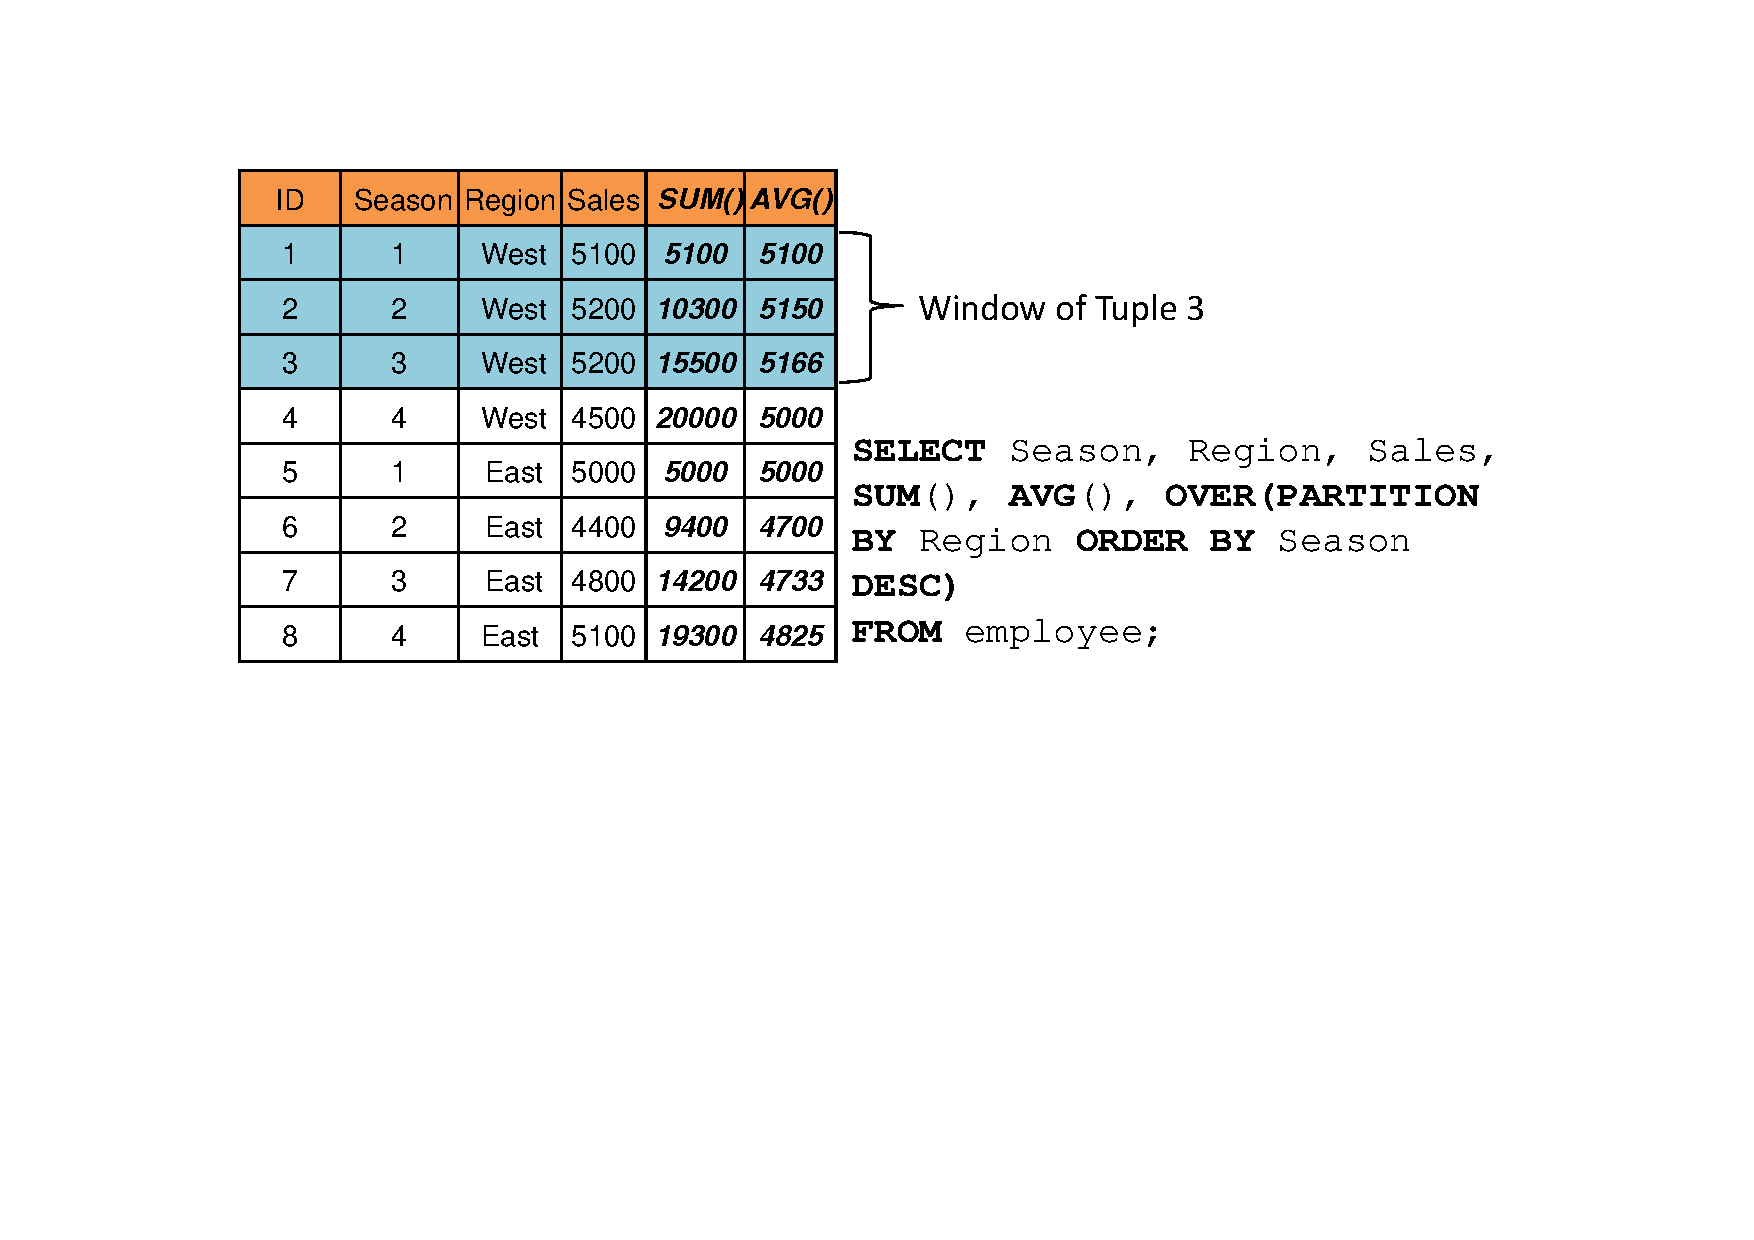
\includegraphics[width=0.8\linewidth]{window_example.pdf}
\caption{A SQL window function computing running sum and average of
sales. The window of tuple 3 is highlighted.} 
\label{fig:window}
\end{figure}

As shown in the figure, the sales report contains six columns: ``ID'',
``Season'', ``Region'' and ``Sales'' are the \emph{facts}, ``$\mathtt{sum()}$'' and ``$\mathtt{avg()}$''
are the \emph{analytics} representing the running sum and average. A window function
is represented by the $\mathtt{over}$ keyword. In this context, the window of a tuple $o_i$
contains other another tuple $o_j$ if $o_i$ and $o_j$ are in the same ``region'' and the``season'' of $o_j$ is
prior to the season of $o_i$. The window of tuple-$3$ is highlighted.
Apart from this example, there are also many other 
usages of the window functions in the relational context~\cite{cao2012optimization}. 
Being aware of the success of the window functions, 
SQL~11~\cite{zemke2012s} standard incorporates ``$\mathtt{LEAD}$'' and ``$\mathtt{LAG}$'' 
keywords to offer fine-grained specifications on a tuple's window.

Despite the usefulness, there are few works reporting
the usage of window functions in data domains such as graphs, sequence data and trajectories.
This may due to the
requirement of \emph{sorting} in the window functions. For example,
in Figure~\ref{fig:window},
objects need to be sorted according to ``Season'', and then the window of
each objects is implicitly formed based on the sorted order. However, 
in other data domains, sorting may be ambiguous and even undefined.

To broaden the usages of the window functions in other data domains, we propose the \emph{neighborhood
analytics} in a more general sense. Given a set of objects 
(such as tuples in relational tables, vertexes in graphs, moving objects in trajectories),
the neighborhood analytics is a composite function
$(\mathcal{F} \circ \mathcal{N})$ applied on every object. Here, $\mathcal{N}$
is the \emph{neighborhood function}, which contains the related objects (i.e., vicinity) of an object;
$\mathcal{F}$ is the \emph{analytic function}, which could be aggregation, ranking,
pattern matching, etc.
Apparently, the SQL window function is a special case of the
neighborhood analytics. For example, the window function in Figure~\ref{fig:window} 
can be represented as $\mathcal{N}(o_i)=\{o_j | o_i.season > o_j.season \wedge o_i.region = o_j.region\}$
and $\mathcal{F} = \mathtt{avg}$.
By relaxing the sorting constraint, neighborhood analytics gains an enriched 
semantic and can be applied on many other data domains.

%Since the \emph{sorting} requirement is relaxed, our neighborhood analytics is able to
%enrich the semantic of relational window notations 
%and can be applied on many other domains.
\section{Thesis Scope}
In this thesis, we explore the neighborhood analytics in emerging applications
from three prevalent data domains, namely \textbf{attributed graph},
\textbf{sequence data} and \textbf{trajectory}. 
To provide useful analytics, we define the following
two intuitive instances of the neighborhood function:
%Since the neighborhood analytics could be very broad,
%this thesis only focus on the following 
%two intuitive neighborhood functions:

\textbf{Distance Neighborhood}: the neighborhood is defined based on numeric distance, that is $\mathcal{N}(o_i,K) = \{o_j | \mathtt{dist}(o_i,o_j) \leq K \}$, where $\mathtt{dist}$ is a distance function and $K$ is a distance threshold.

\textbf{Comparison Neighborhood}: the neighborhood is defined based on the comparison of objects, that is $\mathcal{N}(o) = \{o_i | o.a_m \ \mathtt{cmp} \ o_i.a_m\}$, where $a_m$ is an attribute of object
and $\mathtt{cmp}$ is a binary comparator (i.e., $=,<,>,\leq,\neq,\geq$).

In spite of the simplicity of these two neighborhood functions, they can weave many useful analytics as we shall see in the remaining part of the thesis.
%
%There could be other types of neighborhood functions with different constraints. 
%However, despite the simpleness of these two neighborhood functions, they 
%are indeed versatile in representing many useful analytics.

%In particular, we looked at three most prevalent data domains, namely \textbf{attributed graph},
%\textbf{time series} and \textbf{trajectory}. 
%We then categorize two intuitive neighborhood functions as follows:
%
%\textbf{Distance Neighborhood}: the neighborhood is defined based on numeric distance, that is $\mathcal{N}(o_i,K) = \{o_j | \mathtt{dist}(o_i,o_j) \leq K \}$, where $\mathtt{dist}$ is a distance function and $K$ is a distance threshold.
%
%\textbf{Comparison Neighborhood}: the neighborhood is defined based on the comparison of objects, that is $\mathcal{N}(o) = \{o_i | o.a_m \ \mathtt{cmp} \ o_i.a_m\}$, where $a_m$ is an attribute of object
%and $\mathtt{cmp}$ is a binary comparator.
%
%There could be other types of neighborhoods with more fine-grained or more general definitions. 
%In this thesis, we demonstrate
%that these two simple neighborhood definitions
%joint with traditional analytic functions are already versatile 
%in various domains. 
%\revised{They are cable to both express existing queries and devise novel emerging 
%queries that are practically useful.
%}



\section{Thesis Contributions}
In brief, the contribution of this thesis is twofold.
First, by sewing different $\mathcal{N}$ and $\mathcal{F}$, 
several novel neighborhood based queries are proposed for 
\emph{graph}, \emph{sequence data} and \emph{trajectory} respectively. 
%three interesting
%neighborhood analytic queries are proposed for \emph{graph}, \emph{time series} 
%and \emph{trajectory} domains respectively. 
Second, this thesis
deals with the efficiency issues in deploying the corresponding analytic queries to
handle data of large scale.
The roadmap of this thesis is shown in Figure~\ref{fig:thesis_roadmap}.
\begin{figure}[h]
\centering
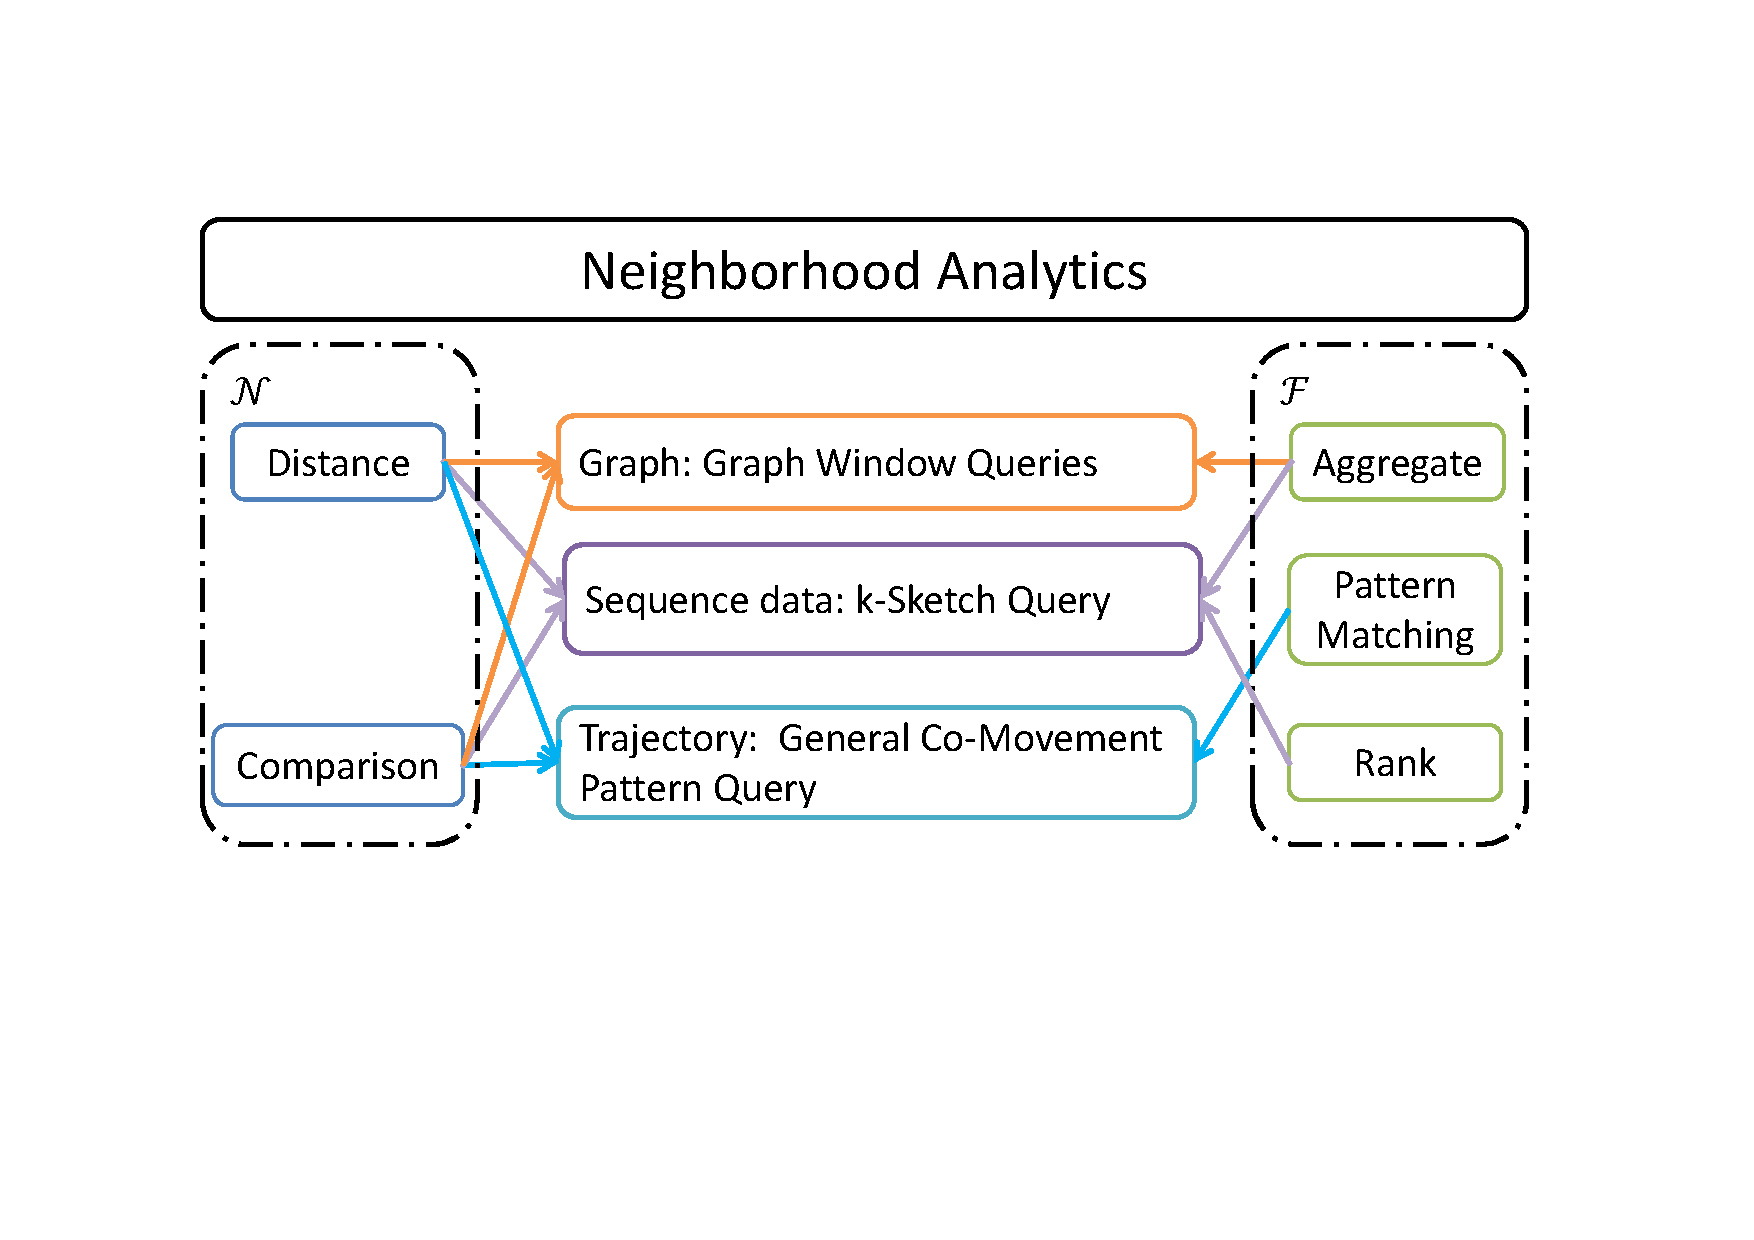
\includegraphics[width=0.8\linewidth]{thesis_roadmap.pdf}
\caption{The roadmap of this thesis. There are three major contributions as highlighted in the center. Each contribution
is an application based on neighborhood analytics with $\mathcal{N}$ and $\mathcal{F}$ as indicated by arrows.} 
\label{fig:thesis_roadmap}
\end{figure}

In a nutshell, we propose three neighborhood based queries in respective data domains. 
In \emph{graph}, we define the Graph Window Query which summarizes the vicinity of each vertex.
The query utilizes both distance neighborhood and comparison neighborhood to facilitate both
general graphs and direct acyclic graphs.
%
%two types of queries: \emph{k-hop window query} is based on the \emph{distance} neighborhood
%and \emph{topological window query} is based on the \emph{comparison} neighborhood. 
In \emph{sequence data}, we propose a $k$-Sketch Query to summarize a subject's history. The $k$-Sketch query builds on a nested \emph{distance} and \emph{comparison} neighborhood based pattern called \emph{rank-aware streak}.
%
% we design a nested \emph{distant} and \emph{comparison} neighborhoods based pattern called \emph{rank-aware streak}, and propose a $k$-Sketch query to select the most representative rank-aware streaks.
In \emph{trajectory}, we propose a General Co-movement Pattern (GCMP) query to discover co-moving behaviors among moving objects. The GCMP query leverages the neighborhood notion to unify existing co-moving patterns in the literature.
%
%we analyze existing movement patterns based
%on \emph{distance} and \emph{comparison} neighborhoods and unify
%the existing works with a general pattern discovery query. 
In the following parts of this section, we present our contributions in detail.


\subsection{Graph Window Queries}
The first piece of the thesis deals with neighborhood analytics
on graph data. Nowadays information network are typically
modeled as attributed graphs where the 
vertexes correspond to objects and the edges capture the
relationships among these objects. As vertexes embed a wealth
of information (e.g., user profiles in social networks), there are 
emerging demands on analyzing these data to extract useful insights. 
We propose the concept of \emph{window analytics} 
for attributed graph and identify two types of such analytics as shown in the following examples:

\textbf{$k$-hop Window:} The $k$-hop neighbors of a vertex form
its $k$-hop window. Since the $k$-hop neighbors are the most structurally
relevant vertexes to the vertex, analytics on the information from the $k$-hop window
would be beneficial. Typical analytic queries include summarizing the related connections' distribution among different companies, and computing age distribution of the related friends can be useful.
%In a social network (such as LinkedIn and Facebook etc.), users are normally modeled as vertexes and connectivity relationships are modeled as edges. In the social network scenario, it is of great interest to summarize the most relevant connections to each user such as the neighbors within $2$-hops. Some analytic queries such as summarizing the related connections' distribution among different companies, and computing age distribution of the related friends can be useful. In order to answer these queries, collecting data from every user's neighborhoods within 2-hop is necessary.
%\end{example}

\textbf{Topological Window:} The topological neighbors are defined
in the context of Directed Acyclic Graph (DAG). In DAGs,
topological neighbors are composed of all the ascendant vertexes of a vertex. 
The topological neighbors represent the most influential vertexes of a given vertex.
Since DAGs are often found in biological networks, topological window would
be helpful to analyze the statistics of molecules of each biological protein's pathway.
%Since the topological neighbors , analytics
%on the topological window would benefit the deeper understanding of the 
%network.
%DAGs are often found
%in biological networks and citation networks. 
% The topological neighbors
%represent the influences from the source vertex to the given vertex, thus
%analytics over topological window would be interesting.

%\begin{example}[Topological window]
%In biological networks (such as Argocyc, Ecocyc etc.), genes, enzymes and proteins are vertexes and their
%dependencies in a pathway are edges. Because these networks are directed and acyclic, 
%in order to study the protein regulating process, one may be interested to find out the statistics of molecules in each protein production pathway. For each protein,we can traverse the 
%graph to find every other molecules that are in the upstream of its pathway.
%Then we can group and count the number of genes and enzymes among those molecules.
%\end{example}

The two \emph{windows} shown in the above examples are essentially neighborhood functions defined for each vertex. Specifically, let $G=(V,E,A)$ be an attributed graph, where $V$ is the set of vertexes, $E$ is the set of edges, and each vertex $v$ is associated as a multidimensional point $a_v \in A$ called attributes.
The \emph{k-hop} window is a \emph{distance} neighborhood function, 
i.e., $\mathcal{N}_1(v,k)= \{u|\mathtt{dist}(v,u) \leq k\}$, 
which captures the vertexes that are $k$-hop nearby. 
The \emph{topological} window,  $\mathcal{N}_2(v)= \{u | u \in v.ancestor\}$,
is a \emph{comparison} neighborhood function that captures
the ancestors of a vertex in a directly acyclic graph.  The analytic function $\mathcal{F}$ is an aggregate function ($\mathtt{sum}$, $\mathtt{avg}$, etc.) on $A$.

Apart from demonstrating the useful use cases on these two windows, 
we also investigate how Graph Window Query processing can be efficiently supported.  We propose
two different types of indexes: Dense Block Index (DBIndex)
and Inheritance Index (I-Index). The DBIndex and I-Index
are specially optimized to support $k$-hop window and topological
window processing. These indexes
integrate the aggregation process with partial work sharing techniques
to achieve efficient computation.
In addition, we develop space and performance efficient techniques
for the index construction. Notably, DBIndex saves upto 80\%
of the index construction time as compared to the state-of-the-art competitor and up to 10 times
speedup in query processing. 


\subsection{$k$-Sketch Query on Sequence Data}
The second piece of this thesis explores the neighborhood analytics on sequence data. 
%In sequence data analysis, 
As part of the sequence data analysis,
summarizing a subject's history with sensational patterns
is an important and revenue-generating task in a plethora of applications 
such as computational journalism~\cite{cohen2011computational,zhang2014discovering}, automatic fact checking~\cite{hassan2014data,walenz2014finding}, and perturbation analysis~\cite{Walenz:2016:PAD:3007328.3007330}.
%
%an important and revenue-generating task is to
%summarize a subject's history using sensational patterns.
An outstanding example of such patterns is the \emph{streak}~\cite{zhang2014discovering},
which is commonly found in stock
and sports reports. For instance:

%For example, streaks may be of the following forms in stock and sports scenarios:

%Streak is commonly used in many sequenced applications,
%such as network monitoring, stock analysis
%and sport reporting. For example, streaks may be of the following forms in stock and sports scenarios:
\begin{enumerate}
	\item{[STOCK]:``Apple Inc.~has an \emph{average} price of USD 115.5 in the \emph{last week}''}
	\item{[SPORTS]: ``Kobe has scored \emph{at least} 60 points in \emph{three straight games}'' }
\end{enumerate}
In general, a streak is constructed from two concepts: an \emph{aggregate function} (e.g., $\mathtt{avg}$, $\mathtt{min}$)
applied on \emph{consecutive events} (e.g., seven days, three games). 
%Indeed, a streak an be simply modeled as a neighborhood query.
However, the streak itself does not embed the strikingness information, which is limited
to represent a sensational pattern. 
%
%
%is a neighborhood query defined for an event where the neighborhood range is the window the event belongs to.
%%
%, a \emph{streak} can be modeled as a neighborhood query
%of events, where the neighborhood function is defined as windows.
%This makes the streak as a neighborhood query of events where the neighborhood function is defined as time windows.
%
%Since the streak is aggregated based on the
%closeness of events in the time domain (i.e., time window), it can be viewed as a neighborhood query where the neighborhood function is defined by the time distance, and the analytic function can be any aggregate function.
%However, it is challenging to directly leverage streaks to discover sensational patterns because
%the strikingness of a streak is missing.
%A direct challenge in discovering phenomenal patterns using streak is
%how to quantify the strikingness of a streak.
For example, \emph{Streak 2} would not be striking if all NBA players were able to score over 60 points. 
On the contrary, knowing that most NBA players only score 20 points in a game,
\emph{Streak 2} is indeed quite striking. 
Therefore, the strikingness of a streak should be measured by comparing with other streaks.
Based on this observation, we propose a rank-aware pattern named \emph{ranked-streak} which measures the strikingness of
a streak by comparing among all streaks under the same condition (i.e., streak length).

Technically, the ranked-streak can be viewed as a joint neighborhood function. 
Let $t_s(e)$ be the sequence number of the event $e$ in the history of subject $s$.
%Let $e_s(t)$ denote the event of subject $s$ at time $t$. 
Then the ranked-streaks of length $L$ are generated using neighborhood functions in a two-step manner: 

\begin{enumerate}
\item {a \emph{distance neighborhood} $\mathcal{N}_1(s,e,L)=\{e_j | t_s(e) - t_s(e_j) \leq L \}$ groups a consecutive $L$ events for each event in the history of subject $s$. Let $\overline{v}$ be the aggregate value associated with $\mathcal{N}_1$, then the output of this step is a set of \emph{streak}s of the form  $sk=\langle s, L, t, \overline{v} \rangle$.}
\item {a \emph{comparison neighborhood} $\mathcal{N}_2(sk) = \{sk_i | sk.L = sk_i.L \wedge sk_i.\overline{v} \geq sk.\overline{v} \}$ ranks a subject's streak among all other streaks with the same length.  Note that the rank information can be simply calculated from a $\mathtt{count}$ function. The result of this step is a tuple $\langle s, L, t, \overline{v}, r \rangle$, where $r$ is the \emph{rank}.}
\end{enumerate}
%(1) a \emph{distance neighborhood} $\mathcal{N}_1(o_i,w)=\{o_j | o_i.t - o_j.t \leq w \}$ groups a consecutive $w$ events for each event. Let $\overline{v}$ be the aggregate value associated with $\mathcal{N}_1$, then the output of this step is a set of \emph{streak}s of the form  $n=\langle o_i, w, t, \overline{v} \rangle$.
%
%(2) a \emph{comparison neighborhood} $\mathcal{N}_2(n_i) = \{n_j | n_j.w = n_i.w \wedge n_i.\overline{v} \geq n_j.\overline{v} \}$ ranks a subject's streak among all other streaks with the same window length. The result of this step is a tuple $\langle o_i, w, t, r \rangle$, where $r$ is the \emph{rank}.
%

As the ranked-streak contains the relative position of the streak among its cohort, it provides a quantitative measure of the strikingness.
For example, the rank-aware version of \emph{Streak 2} would be ``Kobe has scored at least 60 points in three straight games, which is best in the league''.  This clearly suggests that \emph{Streak 2} is striking.
%

On the basis of the ranked-streaks, we study the problem of effectively summarizing
a subject history. We notice that, for a subject with $n$ events, there
are $O{n \choose 2}$ streaks. 
In real life, ``Kobe'' has played $1,000$ games which may produce near half million streaks.
Such a large number of streaks is too overwhelming to represent a subject's history. Hence,
we are motivated to propose a $k$-Sketch query that selects $k$ ranked-streaks which best represent
a subject's history. To find the qualified streaks, we design a novel scoring which
considers both the events covered of the streaks and the ranks of the streaks.
% under a novel scoring function. Our scoring function
%considers both the events covered of the streaks and the ranks of the streaks.

%A prominent drawback of streak is that the amount of streaks
%%Another challenge  the pattern discovery is that the amount of streaks
%for a subject is huge. For a subject with $N$ events,
%there are $O{N\choose 2}$ streaks as well as rank-aware streaks. 
%In real life, ``Kobe'' has played $1000$ games which may produce near half million streaks.
%Such a large number clearly poses difficulties for pattern discoveries.
%%for selecting phenomen streaks. 
%Nevertheless, we observe that many streaks share almost identical information. For example, when Kobe scored 81 points
%in one game, this single-event streak ranks number 1 among all streaks. Subsequently, the streaks with size 3 (i.e., 3 straight games afterwards) ranked number 10. Thus reporting this
%streak only provide redundant striking information (i.e., the 81 point game).
%Based on this observation, we
%propose a $k$-Sketch query to select the $k$ most \emph{representative streaks} via a novel scoring function that considers both strikingness and diversity of streaks.
%
%Our $k$-Sketch query is based on a novel scoring function that consider both the 
%stringness and the diversity of the streaks. 

In this thesis, we extensively study
the technical issues in processing $k$-Sketch queries in both online and offline scenarios.
In the offline scenario, we design two pruning techniques which largely
reduce the streaks enumerated in generating ranked-streaks. Then, we adopt a
$(1-1/e)$-approximate sketch selection algorithm by utilizing the 
submodularity of the $k$-Sketch query. In the online scenario, we design
an \emph{online-streak bound} to avoid evaluating many unnecessary streaks. Furthermore,
we propose a $1/8$-approximate algorithm to facilitate efficient sketch maintenance.
In the experimental study, we compare our solutions with baselines using
four real datasets, and the results demonstrate the efficiency and 
effectiveness of our proposed algorithms: the running time
achieves up to 500 times speedup as compared to the baseline and the quality of the
detected sketch is endorsed by the anonymous users
from Amazon Mechanical Turk\footnote{\url{https://requester.mturk.com}}. 
%
%, our techniques is confirmed by the experiments on four 
%real datasets. And the effectiveness of our $k$-Sketch query is endorsed
%by the anonymous users from Amazon Mechanical Turk\footnote{\url{https://requester.mturk.com}}.

%%
%%Besides proposing the rank-aware streak, we also technically 
%%study how to efficiently support the \emph{$k$-Sketch} query in both
%%offline and online scenarios. We propose various window-level 
%%pruning techniques to find striking candidate steaks.
%%Among those candidates, we then develop approximation
%%methods, with theoretical bounds, to discover $k$-sketches for each subject. 
%Furthermore, we conduct experiments on four real
%datasets, and the results demonstrate the efficiency and 
%effectiveness of our proposed algorithms: the running time
%achieves up to 500x speedup as compared to baseline and the quality of the
%detected sketch is endorsed by the anonymous users
%from Amazon Mechanical Turk \footnote{\url{https://requester.mturk.com}}.

\subsection{Co-Movement Pattern Query on Trajectory Data}
The third piece of the thesis studies the neighborhood
analytics in the trajectory domain. 
In trajectory analysis, an important
mining task is to discover traveling patterns among moving objects. 
A traveling pattern is often determined by the spatial neighborhoods of moving objects. One of the prominent examples is the \emph{co-movement pattern}~\cite{li2013onlinegroup,zheng2015trajectory}.
A co-movement pattern refers to a group of moving objects traveling together for a certain period of time. 
We observe that the co-movement pattern can be concisely represented using two neighborhood functions in spatial and temporal domains as follows:

%Table~\ref{tbl:intro-move-patterns} summarizes several popular co-movement patterns with different 
%constraints with respect to clustering in spatial proximity, consecutiveness in temporal duration
%and computational complexity. In particular, the flock~\cite{gudmundsson2006computing} and the group~\cite{wang2006grouppattern} patterns require all the objects in a group to be enclosed by a disk with radius $r$;
%whereas the convoy~\cite{jeung2008discovery}, the swarm~\cite{li2010swarm} and the platoon~\cite{li2015platoon} patterns resort to density-based spatial clustering. In the temporal dimension,
%the flock~\cite{gudmundsson2006computing} and the convoy~\cite{jeung2008discovery} require all the timestamps
%of each detected spatial group to be consecutive, which is referred to as global consecutiveness; whereas the swarm~\cite{li2010swarm} does not impose any restrictions. 
%The group~\cite{wang2006grouppattern} and the platoon~\cite{li2015platoon} adopt 
%a compromised approach by allowing arbitrary gaps between consecutive segments, 
%which is called local consecutiveness. They introduce a parameter $L$ to control the minimum length of each local consecutive segment.
%
%
%\begin{table}[h]
%\centering
%\begin{tabular}{|l|c|c|}
%\hline 
%\textbf{Pattern} & {\textbf{Proximity}} & { \textbf{Consecutiveness}} \\% & { \textbf{Time  Complexity}}\\ 
%\hline 
%flock~\cite{gudmundsson2006computing} & disk based &  global \\%& {$O(|\mathbb{O}||\mathbb{T}|\log(|\mathbb{O}|))$} \\ 
%\hline 
%convoy~\cite{jeung2008discovery} & density based &   global \\%& {$O(|\mathbb{O}|^2+|\mathbb{O}||\mathbb{T}|)$}\\ 
%\hline 
%swarm~\cite{li2010swarm} & density based  & - \\%& {$O(2^{|\mathbb{O}|}|\mathbb{O}||\mathbb{T}|)$}  \\ 
%\hline 
%group~\cite{wang2006grouppattern} & disk based &  local \\%& {$O(|\mathbb{O}|^2|\mathbb{T}|)$}\\ 
%\hline 
%platoon~\cite{li2015platoon} & density based &  local \\%& {$O(2^{|\mathbb{O}|}|\mathbb{O}||\mathbb{T}|)$}\\ 
%\hline 
%\end{tabular} 
%\caption{Constraints of co-movement patterns.}
%\label{tbl:intro-move-patterns}
%\end{table}
%Neighborhoods relationship
%among moving objects forms the traveling behavior of the objects
%which is often referred as moving patterns. Specifically, the neighborhoods
%of objects are defined based on the spatial proximity and the 
%
%
%nIn trajectory domain, an instance 
%of neighborhood usage is to detect the movement pattern. In simple
%words, a movement pattern is a set of moving object whose trajectories
%exhibits interesting behaviors.
%
%Due to its wide spectrum of applications, 
%mining the movement patterns have attracted many research attention.

%
%In trajectory domain, the neighborhoods of objects across multiple time snapshots collectively 
%form a movement pattern. Due to its wide spectrum of applications, mining the movement patterns have attracted many research attention.
%
%In the trajectory domain, neighborhood
%functions can effectively model the movement patterns
%of objects which is useful in a wide
%spectrum of applications. 
%
%An important mining task in trajectory
%data that has drawn many research attention is discovering
%movement patterns. Coincidentally, a movement pattern
%can be 
%
%
%Discovering co-movement patterns from large-scale trajectory 
%databases is an important mining task and has a wide
%spectrum of applications. 
%Existing studies have identified several types of interesting movement patterns called \emph{co-movement} patterns. A co-movement pattern refers to a group of moving objects traveling together for a certain period of time and the group of objects is normally determined by their spatial proximity. A pattern is prominent if the group size exceeds $M$ and the length of duration exceeds $K$. 
%Inspired by the basic definition 
%and driven by different mining applications, there are a bunch of variant 
%co-movement patterns that have been developed with more advanced constraints.

%\begin{figure}[h]
%\centering
%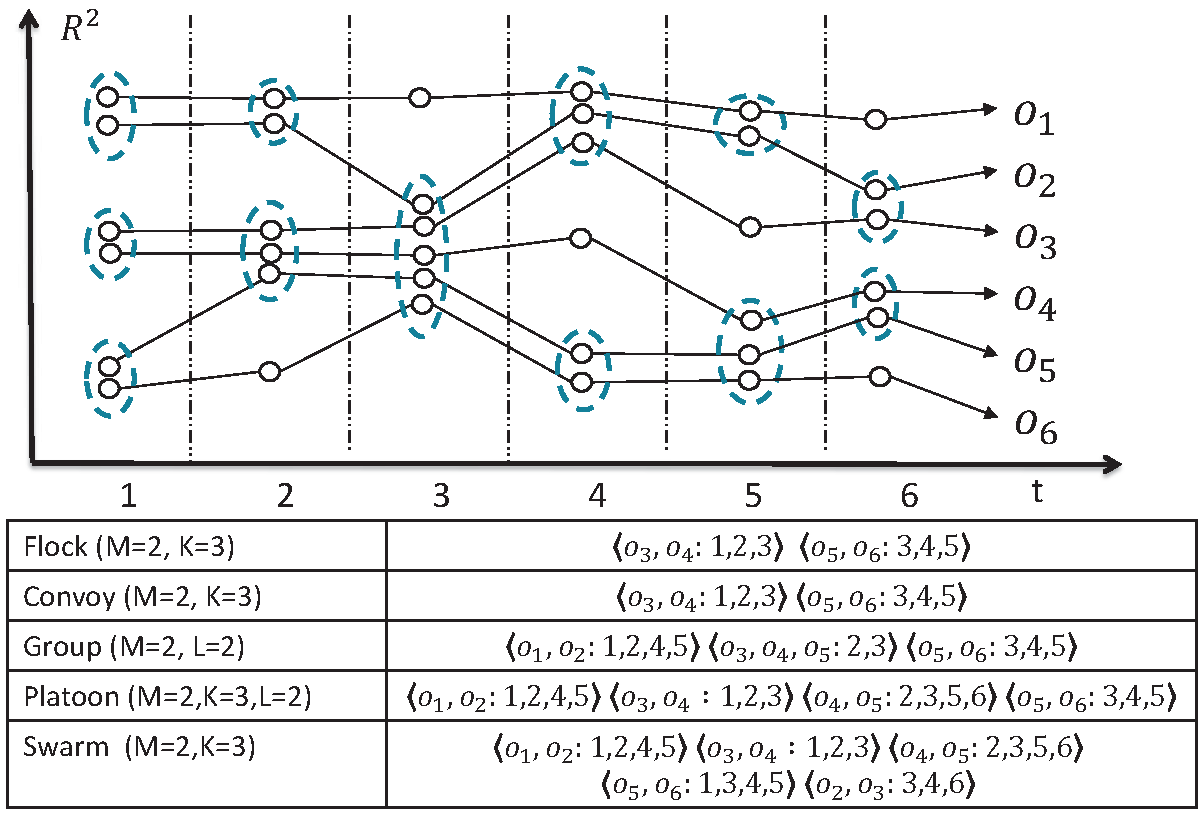
\includegraphics[width=0.8\textwidth]{trajectory_patterns.pdf}
%\caption{Trajectories and co-movement patterns. The example consists of six trajectories across six snapshots. Objects in spatial clusters are enclosed by dotted circles. $M$ is the minimum cluster cardinality; $K$ denotes the minimum number of snapshots for the occurrence of a spatial cluster; and $L$ denotes the minimum length for local consecutiveness.}
%\label{fig:related_work}
%\end{figure}
%
%Figure~\ref{fig:related_work} is an example to demonstrate the concepts of various co-movement patterns. The trajectory database consists of six moving objects and the temporal dimension is discretized into six snapshots. In each snapshot, we treat the clustering method as a black-box and assume that they generate the same clusters. Objects in proximity are grouped in the dotted circles. As aforementioned, there are three parameters to determine the co-movement patterns and the default settings in this example are $M=2$, $K=3$ and $L=2$. Both the \emph{flock} and the \emph{convoy} require the spatial clusters to last for at least $K$ consecutive  timestamps. Hence,$\langle o_3,o_4:1,2,3 \rangle$ and $\langle o_5,o_6:3,4,5 \rangle$  remains the only two candidates matching the patterns. The \textit{swarm} relaxes the pattern matching by discarding the temporal consecutiveness constraint. Thus, it generates many more candidates than the \textit{flock} and the \textit{convoy}. The \textit{group} and the \textit{platoon} add another constraint on local consecutiveness to retain meaningful patterns. For instance, $\langle o_1,o_2:1,2,4,5 \rangle$ is a pattern matching local consecutiveness because timestamps $(1,2)$ and $(4,5)$ are two segments with length no smaller than $L=2$. The difference between the \textit{group} and the \textit{platoon} is that the \textit{platoon} has an additional parameter $K$ to specify the minimum number of snapshots for the spatial clusters. This explains why $\langle o_3,o_4,o_5:2,3 \rangle$ is a \textit{group} pattern but not a \textit{platoon} pattern.


%As shown, there are various types of co-movement patterns facilitating different application needs and 

	(1) In spatial domain, let $o(t)$ be the spatial location of object $o$ at time $t$. The co-moving objects of an object $o$
	can be determined by a \emph{distance neighborhood} $\mathcal{N}_1$. For example,  flock~\cite{gudmundsson2006computing} and group~\cite{wang2006grouppattern} patterns use the \emph{disk-based} clustering, which is equivalent to $\mathcal{N}_1(o, t)= \{o_j | \mathtt{dist}(o(t),o_j(t)) < r \}$. Convoy~\cite{jeung2008discovery}, swarm~\cite{li2010swarm} and platoon~\cite{li2015platoon} patterns use the \emph{density-based} clustering, which is equivalent to $\mathcal{N}_1(o,t)= \{o_j | \mathtt{dist}(o_j(t),o_k(t)) \leq \epsilon \wedge o_k \in \mathcal{N}_1(o,t)\}$.
%	
%	
%	spatial groups of moving objects at time $t$
%	can be formed by a \emph{distance neighborhood} $\mathcal{N}_1$. For example,  flock~\cite{gudmundsson2006computing} and group~\cite{wang2006grouppattern} patterns use the \emph{disk-based} clustering, which is equivalent to $\mathcal{N}_1(o, t)= \{o_j | \mathtt{dist}(o(t),o_j(t)) < r \}$. Convoy~\cite{jeung2008discovery}, swarm~\cite{li2010swarm} and platoon~\cite{li2015platoon} patterns use the \emph{density-based} clustering, which is equivalent to $\mathcal{N}_1(o,t)= \{o_j | \mathtt{dist}(o_j(t),o_k(t)) \leq \epsilon \wedge o_k \in \mathcal{N}_1(o,t)\}$.
%	
%	 $\mathcal{N}_1$ is a \emph{distance neighborhood} used to determine the spatial proximity of objects. For example,  flock~\cite{gudmundsson2006computing} and group~\cite{wang2006grouppattern} patterns uses the \emph{disk-based} clustering, which is equivalent to $\mathcal{N}_1(o, t)= \{o_j | \mathtt{dist}(o(t),o_j(t)) < r \}$ for each object. Convoy~\cite{jeung2008discovery}, swarm~\cite{li2010swarm} and platoon~\cite{li2015platoon} patterns uses the \emph{density-based} clustering, which is equivalent to $\mathcal{N}_1(o,t)= \{o_j | \mathtt{dist}(o_j(t),o_k(t)) \leq \epsilon \wedge o_k \in \mathcal{N}_1(o_i,t)\}$.
	
	(2) In temporal domain, objects that co-move with $o$ for a duration $T$ can be determined by
	a \emph{comparison neighborhood} $\mathcal{N}_2$:
% is a \emph{comparison neighborhood} used to determine co-moving behavior, i.e.,
	%objects that co-move with $o$ for a duration $T$ can be represented by 
	$\mathcal{N}_2(o, T)=\{o_j| \forall t \in T, o_j \in \mathcal{N}_1(o,t) \}$.%, where $C_t(\cdot)$ returns the neighborhoods (i.e., $N_1$) of an object at time $t$.

A pattern is deemed significant if the group size exceeds $M$ (i.e., $|\mathcal{N}_2(\cdot)| \geq M$ and the length of duration exceeds $K$ (i.e., $T \geq K$). 
%The group is defined based on the spatial proximity of objects, which 
%can be seen as the spatial neighbors of each object.
%
%
Rooted from the basic movement definition and driven by different mining applications, there are several instances of co-movement patterns that have been developed with more advanced constraints, namely \emph{flock}~\cite{gudmundsson2006computing}, \emph{convoy}~\cite{jeung2008discovery}, \emph{swarm}~\cite{li2010swarm}, 
\emph{group}~\cite{wang2006grouppattern} and \emph{platoon}~\cite{li2015platoon}. 
However, these solutions are tailored for each individual pattern and it is cumbersome to deploy and optimize each of the algorithms in real applications. Therefore, there 
calls for a general framework which provides versatile and efficient support on these pattern discoveries. 


Towards this goal, we propose a \emph{General Co-Movement Pattern} (GCMP)
query to capture all existing co-movement patterns in one shot. In GCMP, we treat the proximity detection (i.e., $\mathcal{N}_1$) as
a black box and only focus on the pattern detection (i.e., $\mathcal{N}_2$). We relax the parameter settings on the
co-moving duration (i.e., $T$) and by tuning different parameters (as explained in later sections), GCMP
query is able to detect any of the existing patterns.
%
%It is notable that the GCMP
%query is able to detect any of the existing co-movement patterns by adopting different analytic functions.



In the technical aspect, we study how to efficiently process GCMP query 
on the modern parallel processing platform (i.e., Apache Spark) to
gain scalability over large-scale trajectories. 
In particular, we propose two parallel frameworks: (1) TRPM, which partitions trajectories by replicating snapshots in the temporal domain. Within each partition, a line-sweep method is developed to find all patterns. 
(2) SPARE, which partitions trajectories based on object's neighborhood. Within each partitions, a variant of Apriori enumerator is applied to generate all patterns. 
We deploy the two solutions in our in-house cluster with 11 machines. The experiments on three
real trajectory datasets up to 170 million data points confirm the scalability and efficiency 
of our methods.
%
%We then show the efficiency of both our methods in the Apache Spark platform with three real trajectory datasets upto 170 million points. The results show that SPARE achieves upto 14 times efficiency as compared to TRPM, and 112 times speedup as compared to the state-of-the-art centralized schemes.


\section{Thesis Organization}
The remaining part of the thesis are organized as follows: in Chapter 2, we summarize related literature on neighborhood related analytics in different data domains. In Chapter 3, we present the window function on graph data. In Chapter 4, we present a news discovery application on time series data.
In Chapter 5, we present a pattern mining framework on trajectory data. Chapter 6 summarizes this thesis and highlights the future directions.

\chapter{Literature Review}

Lorem ipsum dolor sit amet, consectetur adipiscing elit, sed do eiusmod tempor incididunt ut labore et dolore magna aliqua. Ut enim ad minim veniam, quis nostrud exercitation ullamco laboris nisi ut aliquip ex ea commodo consequat. Duis aute irure dolor in reprehenderit in voluptate velit esse cillum dolore eu fugiat nulla pariatur. Excepteur sint occaecat cupidatat non proident, sunt in culpa qui officia deserunt mollit anim id est laborum.
%\chapter{A General Framework for Discovering Co-movement Patterns in Trajectory Data}


%now enable appendix numbering format and include any appendices
\appendix
\appendix
\section{Proofs of Theorems}
%\subsection{Proof of Theorem~\ref{THM:RP_ETA}} 
%\label{appx:proof-rp-eta}
%\begin{proof}
%We compute $\eta$ by analyzing $\range(\rho_{G,L,K}(\cdot))$.
%In the following, when no ambiguity, we use $\rho(T)$ to represent
%$\rho_{G,L,K}(T)$. For any sequence $T$, its $\rho(T)$ can
%be viewed as interleaving segments and gaps. 
%We may view $\rho(T)$ as $l_1,g_1,\ldots, l_{n-1}, g_{n-1}, l_n$, where $l_i$ is a
%segment and $g_i$ is a gap. For simplicity, we use $l_i$ and $g_i$ directly as their sizes.
%Then the
%range of $\rho(T)$ is $\Sigma_{i=1}^{i=n} l_i + \Sigma_{i=1}^{i=n-1} g_i$. 
%Since $\rho(T)$ is valid, the following constraints holds: 
%(1) $\Sigma_{i=1}^{i=n} l_i \geq K$; (2) $\forall l_i$, $l_i \geq L$;
%(3) $\forall g_i$, $g_i \leq G-1$. Based on constraint (1) and (2), 
%$n \leq \lceil \frac{K}{L}\rceil$. 
%This indicates that $\Sigma_{i=1}^{i=n-1} g_i \leq (\lceil \frac{K}{L}\rceil -1 ) (G-1)$.
%If $l_n > L$ and $\Sigma_{i=1}^{i=n} l_i > K$, we can reduce the range of $\rho(T)$
%by reducing $l_n$. If $\Sigma_{i=1}^{i=n} l_i - K < l_n - L$ 
%then, $\Sigma_{i=1}^{i=n} l_i - K$ can be reduced to $K$. In this case, the maximum range of $\rho(T)$ is 
%$\leq K +(\lceil \frac{K}{L}\rceil -1 ) (G-1)$.
%Otherwise, we can reduce $l_n$ to be $L$. When $l_n = L$, 
%since we wish $\rho(T)$ to be minimum, it indicates $\Sigma_{i=1}^{i=n} l_i \leq K-1$.
%Therefore $\Sigma_{i=1}^{i=n} l_i \leq K-1+L$. In this case,
%the maximum range of  $\rho(T)$ is $K-1+L +(\lceil \frac{K}{L}\rceil -1 ) (G-1)$.
%Taking maximum, the maximal possible $\rho(T)$ for all $T$s is thus $K-1+L +(\lceil \frac{K}{L}\rceil -1 ) (G-1)$. This proves the first half of the theorem.
%
%For the second half of theorem, we prove by construction. Given $G,L,K$, let $\eta^*$
%be the optimal value. Then consider the sequence $T$ generated 
%by replicate the following pattern: a $L$-segment followed by $G$-gap. The replication
%stops when $|T|\geq K$. Apparently $T$ is valid wrt. $G,L,K$.
%It is easy to see that the minimum $\range(\rho(T))$ 
%is $(\lceil \frac{K}{L}\rceil -1 ) (G-1) + K$. Since $\eta^*$ is optimal,
%$\eta^* \geq \range(\rho(T)) = (\lceil \frac{K}{L}\rceil -1 ) (G-1) + K$. Recall $\eta =(\lceil \frac{K}{L}\rceil -1 ) (G-1) + K +L-1$, this implies that $\eta \leq \eta^* + L - 1$. 
%\end{proof}
%\subsection{Proof of Theorem~\ref{THM:RP_ETA}}
%\begin{proof}
%Let $T'$ be the \emph{shortest} valid subsequence (wrt. $K,L,G$) 
%of a valid sequence $T$. Let $\eta$ be the upper bound for all $T'$s among 
%all possible valid sequence. It is easy to see that, under such a setting,
%any valid sequence would be captured by one of the partitions in temporal
%replication. This proves the completeness. Now, we compute the minimum value
%of $\eta$ as follows:
%any $T'$ can be viewed as $n$ consecutive segments with sizes $l_1,..,l_n$
%and $n-1$ gaps with sizes $g_1,...,g_{n-1}$. Since $\eta$ is the upper bond among all $T'$s, $\eta$ can be formulated 
%as follows:
%\begin{equation}
%\eta = \max_{n,l_i,g_i} \{ \Sigma_{i=1}^{i=n} l_i + \Sigma_{i=1}^{i=n-1} g_i \}
%\end{equation}
%With the following constraints: (1)$\forall l_i, L \leq l_i \leq K-1$;(2)
%$\forall g_i, 1 \leq g_i \leq G$; (3) $\Sigma_{i=1}^{i=n} l_i \geq K$ and
%(4) $\Sigma_{i=1}^{i=n-1}l_i  \leq K-1$. The constraint (1)(2)(3) due to the 
%validity of $T'$ and the constraint (4) is because of the minimum size of $T'$.
%Observe that, constraints (1)-(4) form a convex polygon and $\eta$ is monotone
%increasing wrt. $n,l_i,g_i$, the maximum value of $\eta$ is thus taken at the boundaries. Further
%observe that $n \in [2, \lceil \frac{K}{L} \rceil]$ and $K \geq 1$, these
%conditions naturally derive
%$\eta = (\lceil \frac{K}{L} \rceil -1)*G+2K -2$.
%%valid pattern $P$, let $T'$ be the subsequence of $P.T$ which conforms to $K,L,G$ 
%%with the smallest length. Note that there could be many qualified $T'$s. 
%%Let the $i^{th}$ local-consecutive segment of $T'$ be $l_i$ and 
%%let the $i^{th}$ gap of $T'$ be $g_i$. Then, the size of $T'$ can 
%%be written as $\Sigma_i (l_i + g_i)$.  Since $T'$ conforms to $K,L,G$, 
%%then $2K \geq \Sigma_i (l_i) \geq K$, $l_i \geq L$, $g_i \leq G$. 
%%It follows: $\Sigma_i(l_i+g_i) \leq (\lceil \frac{K}{L} \rceil -1) *G+2K$. 
%%If every partition is of at least such a size, then $T'$ must be
%%captured by at least one of the partition. Thus, the pattern $P$ would 
%%be valid in that partition. This proves the completeness.
%\end{proof}
%\subsection{Proof of Theorem~\ref{THM:SPM_CORRECT} and Lemma~\ref{LEM:SPM_CORRECT}}
\vspace{-2mm}
\subsection{Proofs of Theorem~\ref{THM:SPM_LB} and~\ref{THM:SPM_LB_INC}}
\label{apx:thm2proof}
\vspace{-2mm}
\begin{proof}
$\Gamma$ can be formalized using linear algebra:
Let $J$ be the adjacent matrix of $G_A$.
%Let $G_A$ be an aggregated graph, with a $n \times n$ adjacent matrix $J$.
A vertex order on $G_A$ can be represented as 
%
%Since a vertex order is a permutation of $J$, the adjacent matrices 
%of any reordered graphs can be represented as 
$PJP^T$
where $P$ %$\in \mathbb{P}$ 
is a %$n\times n$ 
\emph{permutation matrix}~\footnote{an identity matrix with rows shuffled}.
Consider an assignment matrix $B$ of star partitioning (i.e., $b_{i,j} = 1$ if vertex $j$ is in star $Sr_i$),
$B=\triu(PJP^T)$~\footnote{\text{triu} is the upper triangle part of a matrix} holds.
% $B=\triu(PJP^T)$~\footnote{\text{triu} is the upper triangle part of a matrix}, then $B$ is the assignment matrix of the star partitioning (i.e., $b_{i,j} = 1$ if vertex $j$ is in star $Sr_i$).
%
%In star partitioning, we assign each edge $e(i,j)$ in $G_A$ to the lower vertex, 
%then the matrix $B=\triu(PJP^T)$~\footnote{\text{triu} is the upper triangle part of a matrix}
%represents the assignment matrix wrt. $P$ (i.e., $b_{i,j} = 1$ if vertex $j$ is in star $Sr_i$).
Let vector $\vec{b}$ be the \textit{one}\footnote{every element in $\vec{b}$ is $1$} 
vector with size $n$. Let $\vec{c} = B\vec{b}$, then each $c_i$ 
denotes the number of edges in star $Sr_i$. Thus, $\Gamma$ can be represented
as the infinity norm of $B\vec{b}$. Let $\Gamma^*$ be the minimum $\Gamma$ among all vertex orderings, that is:
\vspace{-1mm}
\begin{equation}
\vspace{-1mm}
\Gamma^* = \min_{P \in \mathbb{P}}{||B\vec{b}||_\infty} \text{ ,where } ||B\vec{b}||_\infty = \max_{1\leq j \leq n}(c_j)
\end{equation}

Let $B^*$ be the optimal assignment matrix. It follows that 
%Since we have a star for each object, by the degree-sum formula and pigeon-hole theorem, 
$\Gamma^*=||B^*\vec{b}||_\infty \geq d/2$.
Next, %for a vertex ordering $P$, 
let $e_{i,j}$ be an entry in $PAP^T$,
% Since  edges in graph $G$ are independent, then
$e_{i,j}$s are independent. Further, $E[\Sigma_{1\leq j \leq n}e_{i,j}]=d$ where $d$ is the average degree of $G_A$.
% Let $d_i$ denote the degree of vertex $i$,
% since a vertex ordering does not
%affect the average degree,
%then $E[d_i]=E[\Sigma_{1\leq j \leq n}e_{i,j}]=d$. 
%Therefore, 
Entries in $B$ can be written as:
\vspace{-4mm}
\begin{equation*}
\vspace{-1mm}
b_{i,j} = \begin{cases}
			e_{i,j}, i>j \\
			0, otherwise
		  \end{cases}  
\end{equation*}

%There are two observations. First, 
%%since $e_{i,j}$s are independent,
%$b_{i,j}$s are independent. Second, 
Since $i>j$ and $e_{i,j}$s are independent. 
$E[b_{i,j}] = E[e_{i,j}]E[i>j]= E[e_{i,j}]/2$.
%As $c_i$ is a sum of $n$ independent 0-1 variables ($b_{i.j}$s).
 By linearity 
of expectations,
we get: $E[c_i] = E[\Sigma_{1\leq j \leq n} b_{i,j}]=E[\Sigma_{1\leq j \leq n} e_{i,j}]/2 = d/2$.
 Let $\mu =E[c_i] = d/2$, 
$t = \sqrt{n\log n}$, by Hoeffding Bound, the following holds:
\vspace{-4mm}
\begin{equation*}
\vspace{-1mm}
\begin{split}
	Pr(c_i \geq \mu + t) &\leq \exp(\frac{-2t^2}{n}) = \exp(-2\log n) = n^{-2}
\end{split}
\end{equation*}

%The first step holds since all $b_{i,j}$ are 0-1 variables. 
Next, the event $(\max_{1 \leq j \leq n}(c_j) \geq \mu + t)$ can be viewed as
$\cup_{c_i} (c_i \geq \mu + t )$, by Union Bound, the following holds:
\vspace{-1mm}
\begin{equation*}
\vspace{-1mm}
\begin{split}
	Pr(\Gamma \geq \mu + t) &=Pr(\max_{1\leq j \leq n}(c_j) \geq \mu + t)  \\
		& = Pr(\cup_{c_i} (c_i \geq \mu + t )) \\
		&\leq \Sigma_{1 \leq i \leq n} Pr(c_i \geq \mu + t) = n^{-1} = 1/n
\end{split}
\end{equation*}
%Substitute back $t$ and $\mu$, we achieve the following concise form:
%\vspace{-1mm}
%\begin{equation*}
%\small
%\vspace{-1mm}
%	Pr(\Gamma \geq (d/2 + \sqrt{n\log n})) \leq 1/n
%\end{equation*}
This indicates the probability of $(\Gamma-d/2) \leq O(\sqrt{n\log n})$ is $(1-1/n)$. 
Since $\Gamma^* \geq d/2$, Theorem 2 holds.
%it follows with probability greater than $(1-1/n)$, 
%$\Gamma - \Gamma^* \leq O(\sqrt{n\log n})$.
When the aggregated graph is \emph{dense} (i.e., $d\geq \sqrt{12 \log n}$),
the Chernoff Bound can be used to derive a tighter bound of 
$O(\sqrt{d\log n}) $ following similar reasoning.
\end{proof}

%\subsection{Proof of Theorem~\ref{THM:SPM_TM}}
%\begin{proof}
%Let $P_1$, $P_2$ be two candidates with $P_1.O \subseteq P_2.O$. It is easy to see that $P_1.T \supseteq P_2.T$.
%Suppose $P_1.T$ cannot be simplified to a candidate sequence. Then
%by proof of contradiction, any subset of $P_1.T$ cannot
%be simplified. It follows that $P_2.T$ cannot be simplified to a candidate sequence. 
%In summary, if $P_1.T$ cannot be simplified, $P_2$ can be pruned. 
%\end{proof}

\subsection{Proof of Theorem~\ref{THM:SPM_CORRECT}}
\label{apx:spm_correct}
\begin{proof}\vspace{-0.5em}
For soundness, let $P$ be a pattern enumerated by SPARE. For any two objects $o_1, o_2 \in P.O$, the edge $e(o_1,o_2)$ is a superset of $P.T$. 
%By the definition of star, $o_1$ $o_2$ belong to the same cluster at every timestamps in $P.T$. 
As $P.T$ is a valid sequence, by the definition of GCMP, $P$ is a true pattern.
For completeness, let $P$ be a true pattern. Let $s$ be the object with smallest ID in $P.O$. We prove that $P$ must be outputted by Algorithm~\ref{algo:apriori_mining} from $Sr_s$. 
First, based on the definition of star, every object in $P.O$ appears in $Sr_s$. Since $P.T$ is decomposable, then by Lemma 3 %$\forall O' \subseteq O$,
the time sequence of %$O'$ 
any subset would not be eliminated by any $\mathtt{sim}$ operations.  Next, we prove at every iteration \emph{level} $\leq |P.O|$, $P.O \subset O_u$, where $O_u$ is the forward closure. We prove by induction. $level$ = 2 trivially holds. If $P.O \subset O_u$ at \emph{level $i$}, then any subsets of $P.O$ with size $i$ are in the candidate set. %In \emph{level} $i+1$, these subsets grow (in last iteration, they grow to $P.O$). 
This suggests that no subsets are removed by Lines~\ref{code:output1-start}-\ref{code:output2-end}. Then, $P.O \subset U_{i+1}$ holds. Since $P.O$ does not pruned by simplification, monotonicity and forward closure, $P$ must be returned by SPARE.
\end{proof}

%next line adds the Bibliography to the contents page
\addcontentsline{toc}{chapter}{Bibliography}
%uncomment next line to change bibliography name to references
%\renewcommand{\bibname}{References}
\bibliography{refs}        %use a bibtex bibliography file refs.bib
\bibliographystyle{plain}  %use the plain bibliography style

\end{document}

